\documentclass[conference]{IEEEtran}
\usepackage{graphicx}
\usepackage{booktabs}
\usepackage{array}
\usepackage{url}
\usepackage{amsmath}

\begin{document}

\title{A Post-Processing Adapter for Correcting False Positives and False Negatives in Egocentric Hand Detection}
\author{
\IEEEauthorblockN{Detection Quality Adapter Project}
\IEEEauthorblockA{Egocentric hand-detection post-processing pipeline}
}

\maketitle

\begin{abstract}
Object detectors operating on video make two kinds of mistakes that are
invisible in a single frame: reporting a hand that is not present (a false
positive) and missing a hand that is (a false negative). Both are detectable
only across multiple frames, since a real hand follows a continuous,
physically plausible trajectory that noise does not. This paper describes a
detection quality adapter: a stateful, six-stage post-processing layer
inserted between a hand detector and its downstream consumers, which
corrects both error types using per-frame geometry and multi-frame tracking,
without retraining or otherwise modifying the detector. The adapter was
built and calibrated against 39 real egocentric work clips (85,784 frames,
153,876 raw detections) spanning 39 distinct jobs, for which no labeled
ground truth exists. In the absence of labels, every threshold was checked
against the dataset's own real distributions rather than set by inspection,
and the pipeline's behavior is further validated through three label-free
evaluations: masked-detection recovery, track-structure analysis, and
per-rule ablation with threshold sensitivity sweeps. The final calibrated
pipeline retains 85.3\% of detections, recovers 2.5\% through interpolation,
and rejects the remainder for cause; masked short-to-medium dropouts (1--10
frames) are recovered at 76--78\% with gracefully degrading localization
accuracy. A depth-based rule for separating a wearer's hands from a
bystander's was found not to generalize across recording batches and is
documented as opt-in rather than shipped by default.
\end{abstract}

\begin{IEEEkeywords}
hand detection, multi-object tracking, false positive rejection, temporal
consistency, egocentric video, stereo depth, post-processing pipeline,
label-free evaluation, ablation study
\end{IEEEkeywords}

\section{Introduction}

A hand detector scoring video frame by frame fails in two directions. A
false positive is a detection reported where no hand is present: a
duplicate box, a bystander's hand, a shadow mistaken for skin. A false
negative is a hand present in the frame that the detector fails to report,
typically during motion blur or a momentary bad frame. False positives
retain footage that should be discarded; false negatives discard footage
that was sound.

Neither error is visible from a single frame. A duplicate box looks like a
normal detection in isolation. A missed hand looks exactly like an empty
frame. The only signal that separates a real detection from a spurious one,
or a genuine gap from a real absence, is behavior across many frames: a
real hand moves along a continuous, physically plausible path, and noise
does not.

The straightforward response --- retrain the detector --- does not fix the
structural problem. A detector scoring one frame at a time has no way to
know that a duplicate should lose to the real hand, because within that
single frame it cannot tell them apart. This work takes the opposite
approach: let the detector over-report (every plausible box, uncapped,
undeduplicated), and place a stateful, multi-frame adapter after it that has
context a single frame never will. This reframes the problem as one of
tracking and consistency, not computer vision. Nothing in the adapter
performs object detection; every stage asks, given noisy boxes over time,
what is the most plausible explanation.

The adapter is specified in two parts. Part 1 defines a generic,
class-agnostic version: four stages of geometric and temporal correction
that require nothing more than per-class size, shape, and speed
expectations. Part 2 specializes it for hands with a low, constantly-reached
instance cap, a head-mounted camera's near-continuous motion, a
characteristic downward exit path, and a second camera view that makes
per-box depth available. This paper covers both parts as built, the real
dataset used to calibrate them, what could and could not be validated in
the absence of labeled ground truth, and three label-free evaluations
designed to characterize the pipeline's behavior without requiring
annotation.

\section{Problem Formulation}

The adapter sits between a detector and everything downstream, and its
contract is deliberately narrow, as summarized in Table~\ref{tab:contract}.

\begin{table}[t]
\caption{The Adapter's Contract, as Specified}
\label{tab:contract}
\centering
\small
\begin{tabular}{@{}p{0.2\linewidth}p{0.7\linewidth}@{}}
\toprule
\textbf{Aspect} & \textbf{Specification} \\
\midrule
Consumes & Per frame, a candidate pool of boxes with confidences, plus frame timestamps \\
Returns & Corrected detections, each marked \emph{reported}, \emph{merged}, \emph{rejected}, or \emph{interpolated} \\
Configured by & Per-class expectations: plausible size, plausible shape, candidate pool size and class maximum, maximum speed, and typical exit behavior \\
Does not & Alter the detector or require retraining. It does ask the detector to stop capping instances itself, and takes over that selection \\
\bottomrule
\end{tabular}
\end{table}

Nothing is ever deleted. A rejected box stays in the record, tagged
untrustworthy rather than removed, for two reasons: every stage's decision
remains auditable after the fact, and a later stage can revise an earlier
tag --- interpolation, for instance, can overwrite a rejected box's position
when the surrounding trajectory supports it. An interpolated detection is an
assertion the adapter made that the detector never did, and downstream
consumers must be able to tell the two apart.

Six classes of false positive are separable without a model, split by
whether they need tracking, listed in Table~\ref{tab:sixclasses}.

\begin{table}[t]
\caption{The Six Separable False-Positive Classes and Their Order of Application}
\label{tab:sixclasses}
\centering
\small
\begin{tabular}{@{}cp{0.16\linewidth}p{0.16\linewidth}p{0.53\linewidth}@{}}
\toprule
\# & Class & Basis & Rejection Criterion \\
\midrule
1 & Duplicate detections & Geometric & Two heavily overlapping boxes on one object --- merge, retain the stronger \\
2 & Implausible size & Geometric & Far larger or smaller than the object can be at working distance \\
3 & Implausible shape & Geometric & Markedly more elongated than the object should be \\
4 & Implausible displacement & Temporal & The box jumps further between consecutive frames than the object can travel \\
5 & Unsupported detection & Temporal & Appears for one or two frames with no track before or after it \\
6 & Static detection & Temporal & Does not move while the camera does, indicating scene structure \\
\bottomrule
\end{tabular}
\end{table}

The split fixes the pipeline's order: the last three rules need tracks, and
tracks only exist after association, so geometric rejection must run before
association, which must run before temporal rejection, which must run
before interpolation. This ordering is also why the instance cap is
deferred rather than applied at the detector. A detector asked to cap
itself selects by confidence within a single frame --- exactly the
comparison that is unreliable, since a duplicate or background object can
outscore a real detection in a given frame, discarding the real one before
the adapter ever sees it. Instead the detector emits a slightly wider
candidate pool, and the adapter selects after association, ranking
candidates by the track supporting them rather than by single-frame score.
This admits more false positives at the input, which is acceptable because
the temporal rules exist to remove them --- but the pool stays narrow, since
a wide one only gives association more spurious candidates to confuse.

\section{System Architecture}

Detections flow through six stages, always in this order (below).
Stages 5 and 6 are hand-specific additions layered on top of the four-stage
generic core.

\begin{center}
\scriptsize
\begin{tabular}{@{}p{0.97\linewidth}@{}}
\hline
\textbf{1 GEOMETRIC REJECTION} --- Duplicate merge $\rightarrow$ size filter $\rightarrow$ shape filter. Per-frame only. \\
\hline
\textbf{2 ASSOCIATION (TRACKER)} --- Greedy nearest-neighbor match against each track's velocity-predicted position. \\
\hline
\textbf{3 TEMPORAL REJECTION} --- Implausible displacement, unsupported flicker, static-against-moving-camera. \\
\hline
\textbf{4 INTERPOLATION AND EXIT DETECTION} --- Exit test first; otherwise fill the gap if resumption matches prediction. \\
\hline
\textbf{5 INSTANCE-CAP SELECTION} (hand-specific) --- Keep the two best-supported tracks, not the two highest-confidence boxes. \\
\hline
\textbf{6 STEREO DEPTH} (hand-specific, opt-in) --- Reject detections farther than arm's reach. Excluded from the default output. \\
\hline
\end{tabular}

\vspace{2pt}
\footnotesize Fig.~1. The six-stage adapter pipeline, applied top to bottom. Order is
load-bearing: stages 3--6 all require tracks, which do not exist until stage 2 has run.
\end{center}

Every detection carries a tag --- \emph{reported}, \emph{merged},
\emph{rejected}, or \emph{interpolated} --- that survives to the final
output, making every stage's decision inspectable after the fact.

\section{Key Design Decisions}

\subsection{Tracking Algorithm: Greedy Nearest-Neighbor, Not Kalman or Hungarian}
The tracker predicts each track's next position by linear extrapolation
from its last known velocity, then matches the nearest detection within a
distance gate. This is deliberately the simplest approach that could work; a
Kalman filter (for a smoothed velocity estimate under sensor noise) and
Hungarian matching (for globally optimal assignment instead of greedy) were
flagged as upgrade paths in code comments but not built, because the simple
version passed every synthetic and real-data test. Premature sophistication
is a cost, not a feature --- the upgrade is built when a real failure
demands it, not speculatively.

\subsection{Identity Signal: Position and Motion Only, Never the Detector's Left/Right Label}
The detector guesses left- or right-hand per box, but that label is least
reliable exactly when it matters most: when two hands cross. The tracker
ignores it entirely for identity decisions, verified with an adversarial
test in which two hands cross with their labels swapped at the crossing
point. An unreliable signal is worse than no signal at all if the system
does not know it is unreliable.

\subsection{Two Gate Radii, Not One}
Early versions used one shared \texttt{max\_speed} value to govern both the
tracker's match gate and Stage 3's displacement-plausibility check. Real
data showed this to be wrong: a genuinely fast hand movement needs a
generous gate so the tracker does not fragment the track, but that same
movement should still be flagged as visually untrustworthy once it is part
of a track. Conflating ``should these be considered the same object'' with
``is this specific frame trustworthy'' is a common tracking bug --- they are
different questions on different timescales. The fields were split into
\texttt{track\_gate\_speed\_px\_per\_frame} (350, generous) and
\texttt{max\_speed\_px\_per\_frame} (110, tightened); see
Section~\ref{sec:calibration} for the effect this had on real tracks.

\subsection{A Generic Core Plus a Thin, Config-Only Hand Layer}
Stages 1--4 know nothing about hands specifically; they are written for any
tracked object with configurable size, shape, and speed expectations. A
\texttt{hand\_config()} function supplies hand-specific numbers, and two
additive stages (selection, stereo depth) sit on top, without any change to
stages 1--4. This is what keeps the generic core testable in isolation and
reusable for a different object class.

\subsection{Calibration Philosophy: Real-Data Checks Over Guesses, Labels Over Both}
Every placeholder threshold was checked against the real dataset's own
distributions before being trusted, using percentiles and structural
invariants rather than visual inspection. A threshold that was a complete
no-op or actively wrong was fixed immediately, without waiting for labeled
ground truth. Anything that genuinely needed labels --- true precision and
recall, candidate-pool-width tuning --- was left alone and documented as
blocked, rather than guessed at. The absence of labels is not the same as
an absence of anything checkable, a claim this paper substantiates further
in Section~\ref{sec:labelfree} with three evaluations that require no
annotation at all.

\section{Dataset}

39 clips, each a distinct real work task, recorded on a head-mounted stereo
camera at 1920$\times$1200, 30~fps, both eyes. Every clip bundle carries
five artifacts: the stereo video pair, raw hand boxes from a fine-tuned
detector (uncapped, undeduplicated, unsmoothed --- deliberately noisy),
full-rate 6-DoF camera pose from onboard visual-inertial odometry,
per-frame timestamps, and task metadata.

\begin{table}[t]
\caption{Dataset Composition}
\label{tab:dataset}
\centering
\begin{tabular}{@{}lr@{}}
\toprule
\textbf{Quantity} & \textbf{Value} \\
\midrule
Clips & 39 \\
Total frames & 85,784 \\
Total raw detections & 153,876 \\
Ground-truth labels available & None \\
2 boxes/frame & 72.3\% \\
1 box/frame & 18.2\% \\
3+ boxes/frame & 5.25\% \\
0 boxes/frame & 4.3\% \\
\bottomrule
\end{tabular}
\end{table}

\emph{Remark:} every one of the 39 clips is a different job --- hairstylist,
carpenter, farmworker, jeweler, mason, mechanic, and others, no repeats
(independently verified: 39 unique values in \texttt{meta.json}'s
\texttt{job} field across all 39 clips). This is why several ``one global
number'' thresholds turned out to be too simple: a farmworker's typical
working distance (median 0.77~m) and a hairstylist's (1.5--1.8~m, arms
extended toward a seated client) are genuinely different populations, not
noise around one true value. This recurs throughout
Sections~\ref{sec:handspec}--\ref{sec:calibration} and again in
Section~\ref{sec:labelfree}.

\section{Hand Specialization}
\label{sec:handspec}

Hands are one configuration of the generic adapter. Most of the
specialization is parameters rather than new logic, but four properties
change behavior materially (Table~\ref{tab:handprops}).

\begin{table}[t]
\caption{Hand-Specific Properties and Their Consequences}
\label{tab:handprops}
\centering
\begin{tabular}{@{}p{0.32\linewidth}p{0.58\linewidth}@{}}
\toprule
\textbf{Property} & \textbf{Consequence for the Adapter} \\
\midrule
At most two instances per frame & The cap is low and constantly reached; the detector requests 3--4 candidates, the adapter selects two after association. \\
Head-mounted camera & The camera moves constantly, so the static-detection rule is unusually discriminating --- with an important exception (Section~\ref{sec:staticbreak}). \\
Characteristic exit path & Hands most often leave downward; the leaving-the-frame test weights the lower border accordingly. \\
A second eye is available & Per-box stereo depth separates the wearer's hands from a bystander's --- the strongest discriminator available, with no equivalent in the generic adapter. \\
\bottomrule
\end{tabular}
\end{table}

Two further properties are easy to assume incorrectly. Hands are roughly
equant, so the shape rule is informative here where it would not be for an
elongated object. And handedness is unreliable exactly when hands cross, so
tracking associates on position and motion, never on the reported label
(Section~IV-B).

\subsection{Duplicate Detection vs.\ Crossing Hands}
The generic dedup rule (Stage 1) merges on IoU alone, before any tracking
exists --- it has no way to know whether two overlapping boxes are one
object detected twice, or two real hands that happen to overlap. A
real-data check across all 39 clips found the discriminator: every real
duplicate pair had a containment ratio (intersection over the smaller
box's area) of at least 0.73 --- one strong box mostly nested inside a
weaker one --- while a synthetic same-size 50\%-overlap crossing sits at
0.5. A \texttt{duplicate\_containment\_threshold} of 0.7 was added for
hands, verified against a pair chosen deliberately in the gap between the
two gates (IoU 0.52, containment 0.68).

\subsection{Where the Static-Detection Assumption Breaks}
\label{sec:staticbreak}
The specification's assumption is that a head-mounted camera moves
constantly enough that a hand is never stationary in the image for a
sustained period. One carpentry clip contradicts this directly: a hand
braced motionless for several seconds while steadying a workpiece, despite
continuous camera motion. Requiring 15 consecutive still-while-moving
frames before rejecting a detection (rather than one) resolved brief real
pauses, but not this multi-second brace. The underlying limitation is
structural: telling a genuine multi-second pause from true background
clutter needs a model that separates rotation-induced apparent motion from
real parallax, not a longer or shorter pixel-threshold window. Section
\ref{sec:ablation} quantifies this rule's overall impact directly: it is the
single largest contributor to rejections of any rule in the pipeline.

\subsection{Stereo Depth: Validated on One Clip, Not on the Dataset}
The ``beyond arm's reach'' rule (Stage 6) was calibrated from a nominal ZED
X stereo model --- 2.2~mm lens, 12~cm baseline, 733~px focal length ---
cross-checked against a real high-confidence box at frame 230 of one clip,
where a disparity of roughly 267~px implied a depth of about 0.33~m,
consistent with that lens's minimum focus distance for a box that large.
Running the same calibration across all 39 clips surfaced a confident false
rejection of the wearer's own hands on a different clip, traced to the
dataset spanning multiple recording batches with different metadata
signatures. Stage 6 is therefore opt-in, invoked only when both video paths
are explicitly supplied, and excluded from the pipeline's default and final
output.

\section{Calibration and Results}
\label{sec:calibration}

The specification's validation section asks for two things: precision and
recall computed per stage, and a labels-free standing check on the
proportion of interpolated detections. Precision and recall are both
defined against ground truth --- whether a box was actually a hand --- and
this dataset has none. The matching machinery to compute them is fully
built and unit-tested against synthetic ground truth, ready the moment a
labeled reference set exists, but it produces no real figure today. What
follows is what was honestly achievable without labels; Section
\ref{sec:labelfree} then goes further, using three evaluations designed
specifically to probe pipeline \emph{behavior} without requiring any
ground truth at all.

\subsection{Threshold Tuning From Real Distributions}
Six thresholds were retuned using percentiles of the real dataset rather
than inspection (Table~\ref{tab:tuning}).

\begin{table}[t]
\caption{Thresholds Retuned from Real, Unlabeled Data Across All 39 Clips}
\label{tab:tuning}
\centering
\small
\begin{tabular}{@{}p{0.24\linewidth}p{0.14\linewidth}p{0.14\linewidth}p{0.36\linewidth}@{}}
\toprule
\textbf{Parameter} & \textbf{Before} & \textbf{After} & \textbf{Evidence} \\
\midrule
plausible\_size & (20,800)px & (50,1150)px & p1=94px, max=1110px \\
plausible\_shape & (0.3,3.0) & (0.5,2.0) & p1=0.54, p99=2.10 \\
max\_dropout\_frames & 10 & 15 & gap-length p75=13 frames \\
max\_speed (plausibility) & 150 px/f & 110 px/f & speed p99.5=97.7 \\
track\_gate\_speed & shared & 350 px/f & above fastest jump (305.8) \\
duplicate\_containment & n/a & 0.7 & duplicates $\geq$0.73, crossings $\sim$0.5 \\
\bottomrule
\end{tabular}
\end{table}

\subsection{Where Every Detection Ends Up}
Across all 39 clips, 153,876 raw detections plus 3,899 Stage-4 fabrications
(157,775 total) give the breakdown in Fig.~\ref{fig:breakdown} by rejection
reason --- a real, unsupervised proxy for where each rule fires, not a
confirmed false-positive rate.

\begin{figure}[t]
\centering
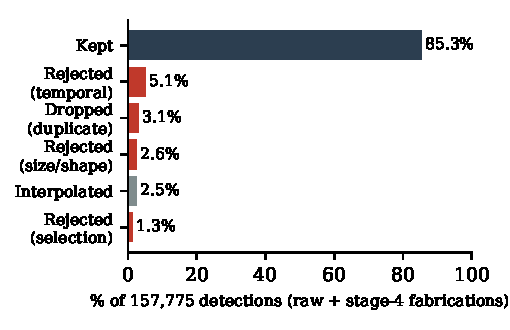
\includegraphics[width=\linewidth]{figures/fig1_rejection_breakdown.pdf}
\caption{Detection outcome breakdown across all 39 clips, reproducible via
\texttt{python calibration/sweep\_thresholds.py --data-dir data} (runtime:
$\sim$4 seconds).}
\label{fig:breakdown}
\end{figure}

\subsection{Final Calibrated Pipeline}
The tuned hand pipeline (Stages 1--5, Stage 6 excluded) produces 148,714
final detections across 787 tracks (Table~\ref{tab:finalresults}).

\begin{table}[t]
\caption{Final Results Across All 39 Clips}
\label{tab:finalresults}
\centering
\small
\begin{tabular}{@{}p{0.52\linewidth}r@{}}
\toprule
\textbf{Metric} & \textbf{Value} \\
\midrule
Final detections (Stages 1--5) & 148,714 \\
Kept & 90.5\% \\
Rejected --- temporal (Stage 3) & 5.5\% \\
Interpolated (Stage 4) & 2.6\% \\
Rejected --- selection (Stage 5) & 1.4\% \\
Dropped as duplicate (Stage 1)* & 3.1\% \\
Rejected --- size/shape (Stage 1)* & 2.6\% \\
Tracks confirmed exiting & 36.1\% \\
Interpolated proportion, mean/max & 3.5\% / 17.2\% \\
\bottomrule
\end{tabular}\\
\raggedright\footnotesize *Measured against all 153,876 raw detections.
\end{table}

\section{Label-Free Behavioral Evaluation}
\label{sec:labelfree}

Rejection-reason frequencies (Section~\ref{sec:calibration}) describe
\emph{where} the pipeline acts but not whether it acts correctly. This
section adds three evaluations that probe pipeline \emph{behavior} using
signals already present in the data --- without requiring any manual
annotation. Each is explicit about what it does and does not establish;
none of them substitutes for true precision/recall against ground truth.

\subsection{Dropout Recovery}
\label{sec:dropout}

\textbf{Method.} For each clip, we identify runs of consecutive, unmodified
detections within a track and artificially delete interior blocks of length
1, 2, 3, 5, 10, and 15 frames, using one centered placement per qualifying
run. The pipeline (Stages 1--4) is then re-run on the masked input from a
fresh clip load, and we measure: the recovery rate (does an
\emph{interpolated} detection reappear at each masked frame), localization
accuracy (IoU and center distance against the deleted box), and the
false-fill rate (spurious interpolation at unmasked neighboring frames).
The deleted box itself is the detector's own (already stage-1--3-filtered)
output, not ground truth, so this measures self-consistency of the
recovery mechanism, not correctness against real hand position.

\textbf{Results.} Recovery rate is flat at 76--78\% for gaps of 1--10
frames, while localization quality degrades smoothly as the gap widens
(median IoU 0.945 at gap~1 down to 0.761 at gap~10; Fig.~\ref{fig:dropout}).
At gap 15, recovery collapses to 9.5\%. This is not noise: at a 15-frame
masked gap, the true distance between surviving anchors is 16 frames, which
exceeds \texttt{max\_dropout\_frames} (15) --- a config field shared
between the tracker's own patience window (\texttt{association.py}) and
Stage 4's fill cutoff (\texttt{interpolation.py}). The tracker itself
expires the track before Stage~4 is ever consulted; the collapse is a
config-coupling artifact, not evidence that 15-frame interpolation is
inherently unrecoverable. False-fill rate stays under 1.2\% throughout.

\begin{figure}[t]
\centering
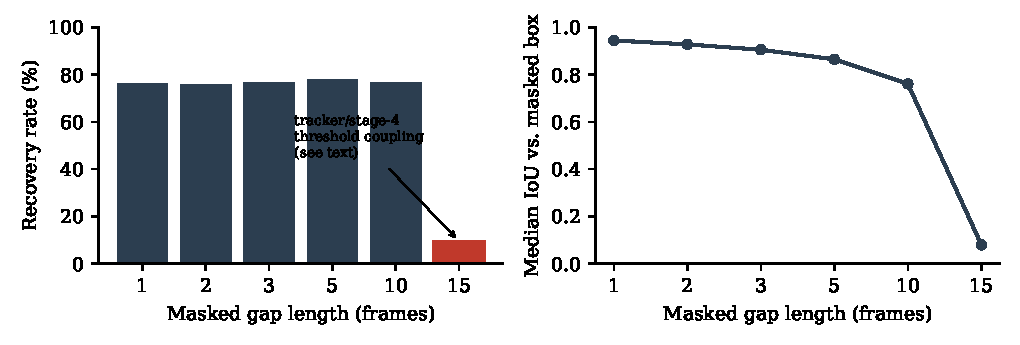
\includegraphics[width=\linewidth]{figures/fig2_dropout_recovery.pdf}
\caption{Recovery rate and median IoU vs.\ masked gap length, pooled across
all 39 clips (1,061--1,815 placements per gap length). Reproducible via
\texttt{python calibration/dropout\_recovery.py --data-dir data}.}
\label{fig:dropout}
\end{figure}

\textbf{What this shows.} The interpolation mechanism recovers a large,
consistent majority of short-to-medium dropouts with position/size accuracy
that degrades gracefully rather than catastrophically, and does so with a
low fabrication rate. It also surfaces a genuine, previously undocumented
coupling: sharing one threshold between the tracker's patience window and
the interpolation cutoff creates a hard reliability cliff exactly at that
threshold. \textbf{What it does not show:} correctness against real hand
position --- a detector systematically wrong in the same way at a masked
frame and at its own interpolation of that frame would score perfectly
here.

\subsection{Track Structure}

\textbf{Method.} We compare ``association only'' (Stages 1--2) against the
full hand pipeline (Stages 1--5) across all 39 clips, measuring track
count, mean track length, a fragmentation proxy (a track starting within 30
frames and 2$\times$ box diagonal of another track's end --- a plausible,
not confirmed, severed continuation), gaps per track, and interpolated
proportion.

\textbf{Results.} Track count (787), mean track length, and the
fragmentation proxy (254 candidates, 28.5\% of tracks) are
\emph{identical} between the two arms. This follows directly from the
pipeline's design: no stage after the tracker (Stage 2) ever merges,
splits, or extends a track's start/end --- Stages 3--5 only tag existing
detections or fill gaps strictly between them. What the correction stages
change is track \emph{content}: total gap-frames drop by 53\% (8,240
$\rightarrow$ 4,341) and interpolated proportion rises from 0.0\% to 3.5\%.

\textbf{What this shows.} The temporal/interpolation/selection stages
operate purely as content-level correctors on top of whatever tracks
association already produced --- they cannot be masking poor tracking by
artificially bridging fragmented tracks into fewer, longer ones, because
track topology is provably unchanged. \textbf{What it does not show:}
whether the association stage's own 28.5\% fragmentation rate is itself
good or bad --- the proxy is a spatial/temporal heuristic, and two distinct
real objects passing through the same location in quick succession would
trigger it identically to a genuinely severed track.

\subsection{Ablation and Sensitivity}
\label{sec:ablation}

\textbf{Method.} Each of the eight per-frame/per-track rules is disabled in
turn via a structural no-op configuration override (e.g.\
\texttt{duplicate\_iou\_threshold=1.1}, an unreachable IoU), and the full
39-clip pipeline is re-run from a fresh load for each configuration
(runtime: 10.7~s for all eight ablations). Separately, eleven thresholds are
swept across 8--9 points spanning a plausible range centered on their
current default (85 full-dataset passes, 116.7~s total), reporting how
kept\% responds.

\textbf{Ablation results.} Fig.~\ref{fig:ablation} ranks the eight rules by
their effect on kept\% when disabled. The static-detection rule (Section
\ref{sec:staticbreak}) is the single largest contributor
(+4.8~pp when disabled), followed by the shape filter (+2.5~pp); the size
filter and flicker/unsupported checks are structurally near-inert
(0.0~pp) on this dataset. Disabling dedup \emph{reduces} kept\% (--2.0~pp)
despite eliminating duplicate rejections outright, because undeduplicated
boxes then compete for Stage 5's fixed 2-instance cap and lose there
instead --- evidence that dedup and selection perform complementary, not
redundant, work. \texttt{max\_dropout\_frames} could not be cleanly
ablated for Stage 4 in isolation, since the tracker reads the same field
for its own patience window (Section~\ref{sec:dropout}); disabling it
(setting it to 0) collapses the tracker itself rather than isolating
interpolation, and is excluded from Fig.~\ref{fig:ablation} for that
reason.

\begin{figure}[t]
\centering
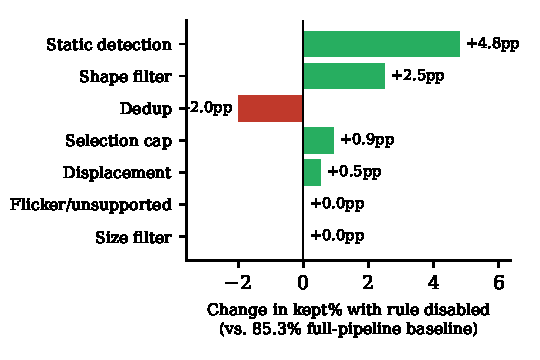
\includegraphics[width=\linewidth]{figures/fig3_ablation.pdf}
\caption{Change in kept\% when each rule is disabled, vs.\ the 85.3\%
full-pipeline baseline. Reproducible via \texttt{python
calibration/ablation.py --data-dir data}.}
\label{fig:ablation}
\end{figure}

\textbf{Sensitivity results.} Table~\ref{tab:sensitivity} and
Fig.~\ref{fig:sensitivity} classify eleven thresholds as sitting on a flat
plateau (small kept\% change across the swept range) or a knife-edge (a
single-step change exceeding 5~pp anywhere in range).
\texttt{track\_gate\_speed\_px\_per\_frame}, \texttt{duplicate\_iou\_threshold},
\texttt{duplicate\_containment\_threshold}, and \texttt{plausible\_size}'s
upper bound are flat --- their current defaults could move substantially
with negligible effect. \texttt{static\_px\_threshold},
\texttt{min\_static\_run\_frames}, \texttt{plausible\_size}'s lower bound,
and both \texttt{plausible\_shape} bounds are knife-edge: exactly the
thresholds where a labeled reference set would matter most, since small
changes there swing outcomes by double-digit percentage points.

\begin{table}[t]
\caption{Threshold Sensitivity Verdicts}
\label{tab:sensitivity}
\centering
\small
\begin{tabular}{@{}p{0.5\linewidth}p{0.12\linewidth}p{0.28\linewidth}@{}}
\toprule
\textbf{Threshold} & \textbf{Default} & \textbf{Verdict} \\
\midrule
max\_speed\_px\_per\_frame & 110 & flat \\
track\_gate\_speed\_px\_per\_frame & 350 & flat \\
max\_dropout\_frames & 15 & knife-edge at 0$\to$1 only \\
min\_static\_run\_frames & 15 & knife-edge \\
static\_px\_threshold & 4.0 & knife-edge \\
duplicate\_iou\_threshold & 0.5 & flat \\
duplicate\_containment\_threshold & 0.7 & flat \\
plausible\_size (lower) & 50 & knife-edge above $\sim$120px \\
plausible\_size (upper) & 1150 & flat \\
plausible\_shape (lower) & 0.5 & knife-edge above $\sim$0.5 \\
plausible\_shape (upper) & 2.0 & knife-edge below $\sim$2.0 \\
\bottomrule
\end{tabular}
\end{table}

\begin{figure}[t]
\centering
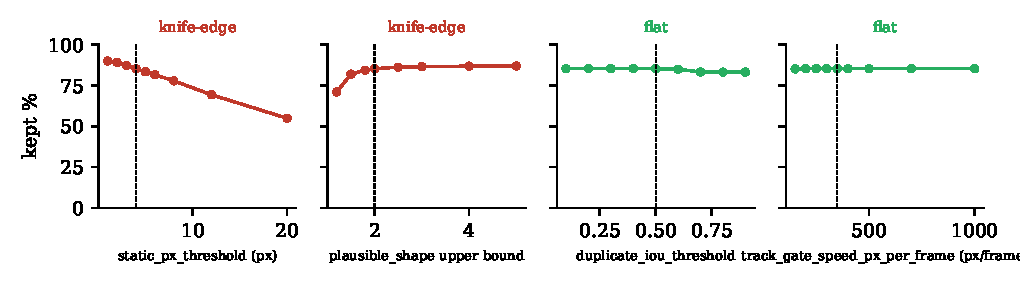
\includegraphics[width=\linewidth]{figures/fig4_sensitivity.pdf}
\caption{Representative sensitivity curves: two knife-edge thresholds and
two flat thresholds. Dashed line marks the current default. Reproducible
via \texttt{python calibration/ablation.py --data-dir data}.}
\label{fig:sensitivity}
\end{figure}

\textbf{What this shows.} Without labels, ablation and sensitivity together
identify which rules and thresholds materially drive outcomes on this
dataset versus which are structurally inert or robust to their exact
setting --- a defensible, if informal, robustness claim for the flat
thresholds, and a concrete prioritization signal for where future labeled
calibration effort matters most. \textbf{What this does not show:}
correctness. A rule firing more or less does not by itself indicate it is
now more or less accurate; ``knife-edge'' flags where the \emph{optimal}
value would matter, not what that value is.

\section{Limitations}

Table~\ref{tab:limitations} summarizes known limitations, updated with the
findings from Section~\ref{sec:labelfree}.

\begin{table}[t]
\caption{Summary of Limitations}
\label{tab:limitations}
\centering
\small
\begin{tabular}{@{}p{0.28\linewidth}p{0.62\linewidth}@{}}
\toprule
\textbf{Limitation} & \textbf{Detail} \\
\midrule
No ground truth & Every number in this paper, including the label-free
evaluations of Section~\ref{sec:labelfree}, is evidence-based or
self-consistency-based, not precision/recall-optimal. \\
Stereo depth does not generalize & Calibrated and validated on one clip;
misjudged depth by roughly 4$\times$ on a different clip. Opt-in, excluded
by default. \\
Multi-second static braces & The largest single driver of rejections
(Section~\ref{sec:ablation}) cannot yet distinguish a multi-second
deliberate hold from background structure. \\
\texttt{max\_dropout\_frames} cross-stage coupling & The same field gates
both the tracker's patience and Stage 4's fill cutoff, producing a sharp
recoverability cliff at the threshold rather than graceful degradation
(Section~\ref{sec:dropout}). \\
One global number for 39 jobs & Arm's reach, camera speed, and hand size
vary by task; a job-aware version was considered and not built, since
deriving a job's normal range from its own detections would be circular
without labels. \\
Greedy, not globally optimal tracking & Nearest-neighbor matching can in
principle mis-assign in dense, ambiguous scenes; not observed in this
dataset, but a known theoretical gap. \\
\bottomrule
\end{tabular}
\end{table}

\section{Conclusion and Future Work}

This paper described a six-stage post-processing adapter that corrects
false positives and false negatives in hand detection using temporal
consistency rather than detector retraining. Beyond the rejection-reason
frequencies used to characterize where the pipeline acts, three label-free
evaluations characterize \emph{how well} it acts without requiring any
manual annotation: dropout recovery shows a consistent 76--78\% recovery
rate with gracefully degrading localization for short-to-medium gaps;
track-structure analysis shows the correction stages cannot be masking
poor tracking, since track topology is fixed entirely by the association
stage; and ablation/sensitivity analysis identifies which rules and
thresholds materially drive outcomes, prioritizing exactly where future
labeled calibration would matter most.

Three lines of work remain, all requiring the labeled reference set the
specification calls for: true per-stage precision and recall,
candidate-pool-width tuning, and validation of a job-aware scaling factor
for the knife-edge thresholds identified in Section~\ref{sec:ablation}. A
fourth line does not require labels but does require new modeling:
separating camera-rotation-induced apparent motion from true parallax, to
resolve the multi-second static-brace failure. A fifth --- decoupling
\texttt{max\_dropout\_frames}'s two roles so that interpolation
reliability degrades smoothly rather than cliff-like at the threshold ---
follows directly from Section~\ref{sec:dropout} and requires no labels at
all. A sixth --- recovering or deriving true per-clip stereo calibration
--- would let Stage 6 move from opt-in to a validated part of the default
pipeline.

\appendix
\section*{Glossary of Terms}
\begin{table}[h]
\centering
\small
\begin{tabular}{@{}p{0.22\linewidth}p{0.68\linewidth}@{}}
\toprule
\textbf{Term} & \textbf{Meaning} \\
\midrule
Detection & One raw box the detector reported on one frame, with a confidence score \\
Track & An ordered sequence of detections believed to be the same physical object over time \\
Tag & What happened to a detection: reported, merged, rejected, or interpolated \\
IoU & Intersection-over-union --- overlap between two boxes, 0 to 1 \\
Disparity & Pixel shift of the same point between stereo views \\
VIO pose & Visual-inertial odometry --- the camera's estimated 6-DoF pose per frame \\
Gate/gating & A maximum-distance cutoff for a plausible track match \\
Standing check & A labels-free monitor --- here, interpolated proportion \\
Knife-edge & A threshold where a small change produces a large ($>$5pp) outcome swing \\
False-fill rate & Rate of spurious interpolation at frames that were not masked/missing \\
\bottomrule
\end{tabular}
\end{table}

\end{document}
